\vspace*{\subsecspace}
\section{Experimental Evaluation}
\label{sec:eval}

%Opening is deliberately short because we gonna be running out of space 
In this section, we present empirical and analytical evaluation of the performance and cost of \sysname under different workloads and scales. 
Our evaluation consists of empirical analysis of the different scientific computing applications, as well as model-driven simulations for analyzing and comparing \sysname behavior under different preemption and application dynamics. 

% \begin{itemize}
% \item What is performance and cost of 
% \end{itemize}

\noindent \textbf{Environment and Workloads:} All our empirical evaluation is conducted on the Google Public Cloud, and with these representative scientific computing applications: 
% open-source
%\vspace*{\tightext}
%\begin{description}
  %TODO: Need MAX two sentence descriptions

\noindent \textbf{Nanoconfinement.}
The nanoconfiment application launches molecular dynamics (MD) simulations of ions in nanoscale confinement created by material surfaces \cite{jyto,kadupitiya2017}.

\noindent \textbf{Shapes.} The Shapes application runs an MD-based optimization dynamics to predict the optimal shape of deformable, charged nanoparticles \cite{jto1,jjzo1}. 

\noindent \textbf{LULESH.} Livermore Unstructured Lagrangian Explicit Shock Hydrodynamics (LULESH) code is a popular code to for hydrodynamics simulations of continuum material models \cite{IPDPS13:LULESH,LULESH2:changes}. 
%\end{description}
%\vspace*{\tightext}

These examples are representative of typical scientific computing applications in the broad domain of physics, materials science, and chemical engineering. These three examples are implemented as parallel programs that use OpenMP and MPI parallel computing techniques. The first two are used in nanoscale materials research \cite{jso1,jso2,solis2013generating,jjzo1,jto1,jyto} and the LULESH is a widely used benchmark \cite{IPDPS13:LULESH,LULESH2:changes}. All applications are run with default parameters unless otherwise stated. 
All applications use OpenMPI, are deployed on Slurm vXXX and 64-bit Ubuntu 18.04, and run on Google Cloud VMs with x86-64 Intel Broadwell CPUs. 
%Networking? 


\vspace*{\subsecspace}
\subsection{SciSpot Performance and Cost}

%%%%%%%%%%%%%%%%%%%%%%%%%%%%%%%%%%%%%%%%%%%%%%%%%%
\subsubsection{Impact of server exploration}

As described in Section~\ref{sec:design}, applications can be deployed on multiple types of VMs in the cloud, with each VM type having a different ``size''.
In our evaluation of parallel scientific computing applications that are CPU intensive, we are primarily interested in the number of CPUs in a VM.

When an application (i.e., bag of jobs) requests a total number of CPUs to run each of its jobs, \sysname first runs its exploration phase to find the ``right'' VM for the application.
\sysname searches for the VM that minimizes the total expected cost $E[C_{(i,n_i)}]$ of running the application, and this depends on several factors such as the parallel structure of the application, the preemption probability and the associated job recomputation time, and the price of the VM.

Thus, even if the \emph{total} amount of resources (i.e., number of CPUs) per job is held constant, the total running time of an application depends on the choice of the VM type ($i$), and the associated number of VMs ($n_i$) required to meet the allocation constraint (Section~\ref{subsec:cost-model}).
%
With preemptible instances, the total running time of a job is composed of two factors: the ``base'' running time of the job without any preemptions ($T_{(i,n_i)}$), and the expected recomputation time which depends on the probability of job failure (Equation~\ref{eq:et1}). 

\begin{figure}
  \centering
  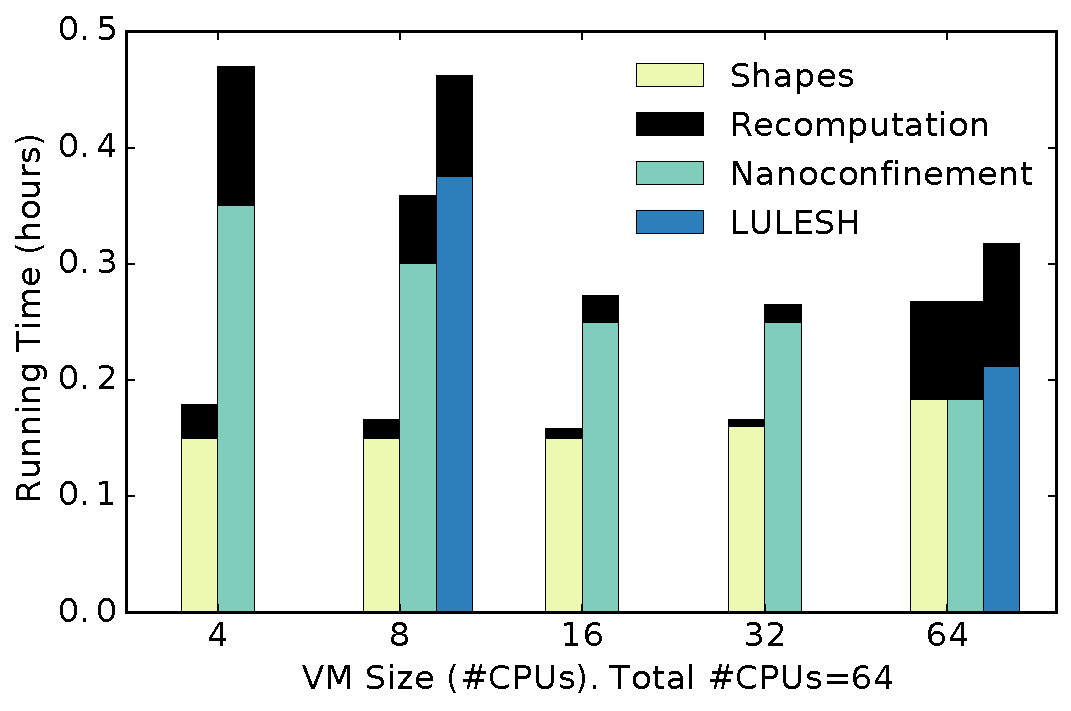
\includegraphics[width=0.4\textwidth]{../graphs/runtime-bars.pdf}
      \vspace*{\myfigspace}
  \caption{Running times of applications on different VMs. The total number of CPUs is 64, yielding different number of VMs in each case. We see different tradeoffs in the base running times and recomputation costs for the different applications.}
  \label{fig:runtimes-bar}
    \vspace*{\myfigspace}
\end{figure}


Figure~\ref{fig:runtimes-bar} shows the running times of the Nanoconfinement and Shapes application, when they are deployed on different VM sizes.
In all cases, the total number of CPUs per job is set to 64, and thus the different VM sizes yield different cluster sizes (e.g., 16 VMs with 4 CPUs or 32 VMs with 2 CPUs).


For the Nanoconfinement application, we observe that the base running times (without preemptions) reduce when moving to larger VMs, because this entails lower communication costs.
The running time on the ``best'' VM (i.e., with 32 CPUs) is nearly 40\% lower as compared to the worst case. 
On the other hand, the Shapes application can scale to a larger number of VMs without any significant communication overheads, and does not see any significant change in its running time.

Figure~\ref{fig:runtimes-bar} also shows the total expected running time $E[T_{(i,n_i)}]$, that is obtained by adding the the expected recomputation time, which depends on the expected lifetimes of the VM and the number of VMs, and is computed using the cost model introduced in Section~\ref{subsec:cost-model}. 
While selecting larger VMs may reduce communication overheads and thus improve performance, it is not an adequate policy in the case of preemptible VMs, since the preemptions can significantly increase the total running time.
We can observe this in the case of Nanoconfinement application when deployed on a 64 CPU VM---even though the base running time is lower compared to deploying the application on 2x32-CPU VMs, the recomputation time on the 64 CPU VM is almost $4\times$ higher due to the much lower expected lifetime of the larger VMs. 
Thus, on preemptible servers, there is a tradeoff between the base running time which only considers parallelization overheads, and the recomputation time.
By considering \emph{both} these factors, \sysname's server selection policy can select the best VM for an application. 


\noindent \emph{\textbf{Result:} SciSpot's server selection, by considering both the base running time and recomputation time, can improve performance by up to 40\% , and can keep the increase in running time due to recomputation to less than 5\%.}

%%%%%%%%%%%%%%%%%%%%%%%%%%%%%%%%%%%%%%%%%%%%%%%%%%
\subsubsection{Cost}

\begin{figure}
  \centering
  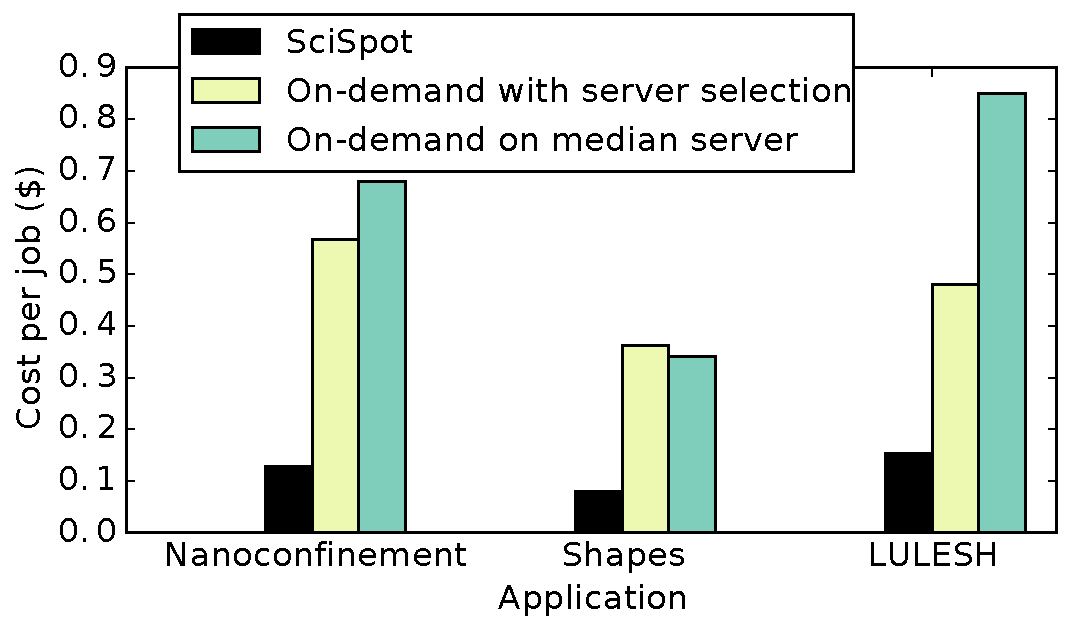
\includegraphics[width=0.4\textwidth]{../graphs/cost-only-bar.pdf}
  \vspace*{\myfigspace}
  \caption{SciSpot's use of preemptible VMs can reduce costs by up to $5\times$ compared to conventional cloud deployments.}
  \label{fig:cost-only-bar}
    \vspace*{\myfigspace}
\end{figure}


The primary motivation for using preemptible VMs is their significantly lower cost compared to conventional ``on-demand'' cloud VMs that are non-preemptible. 
Figure~\ref{fig:cost-only-bar} compares the cost of running different applications with different cloud VM deployments.
\sysname, which uses both cost-minimizing server selection, and preemptible VMs, results in significantly lower costs across the board, even when accounting for preemptions and recomputations. 
Even with \sysname's server selection, using on-demand VMs result in a $5\times$ cost increase compared to \sysname.
In the absence of server selection, we assume that the user will pick a ``median'' VM in terms of number of CPUs (in this case, 8 CPU VMs), which we also show in Figure~\ref{fig:cost-only-bar}.
Note that since \sysname's server selection considers the total turnaround time (which includes recomputation time), it may not always pick the optimal on-demand server. 

%\vj{Note that \sysname's server selection considers both the base running times and recomputation time, which may not necessarily yield the best on-demand server configuration (which only needs to be cognizant of the base running times), and thus we see that the cost for the Shapes application on the median on-demand server is slightly lower than one with \sysname's server selection. However, it is still lower than \sysname's cost. rephrase}


\noindent \emph{\textbf{Result:} SciSpot reduces computing costs by up to 5$\times$ compared to conventional on-demand cloud deployments.}

%%%%%%%%%%%%%%%%%%%%%%%%%%%%%%%%%%%%%%%%%%%%%%%%%%
\subsubsection{Comparison with HPC Overhead}

Scientific applications are typically run on large-scale HPC clusters, where different performance and cost dynamics apply.
While there are hardware differences between cloud VMs and HPC clusters that can contribute to performance differences, we are interested in the performance ``overheads''.
In the case of \sysname, the job failures and recomputations increase the total job running time, and are thus the main source of overhead.

On HPC clusters, jobs enjoy significantly lower recomputation probability, since the hardware on these clusters has MTTFs in the range of years to centuries~\cite{dongarra-ckpting}.
However, we emphasize that there exist \emph{other} sources of performance overheads in HPC clusters.
In particular, since HPC clusters have high resource utilization, they also have significant \emph{waiting} times. 
On the other hand, cloud resource utilization is low~\cite{borg} and there is usually no need to wait for resources, which is why transient servers exist in the first place. 


Thus, we compare the performance overhead due to preemptions for \sysname, and job waiting times in conventional HPC deployments.
To obtain the job waiting times in HPC clusters, we use the LANL Mustang traces published as part of the Atlas trace repository~\cite{cmu-atlas}.
We analyze the waiting time of over two million jobs submitted over a 5 year period, and compute the increase in running time of the job due to the job waiting or queuing time. 

\begin{figure}[t]
  \centering 
  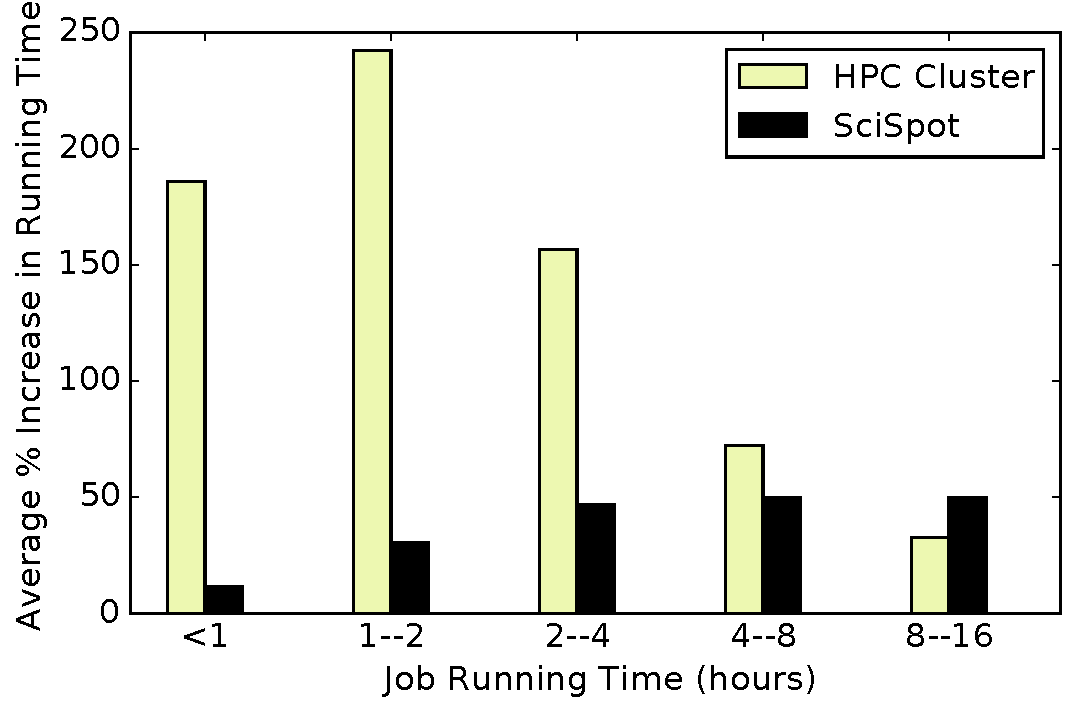
\includegraphics[width=0.4\textwidth]{../graphs/hpc-vs-scispot.pdf}
      \vspace*{\myfigspace}
  \caption{Increase in running time due to waiting/queuing on HPC clusters is significantly higher than the recomputation time for \sysname, especially for shorter jobs. }
  \label{fig:hpc-vs-scispot}
  \vspace*{\myfigspace}
\end{figure}


We define the overhead as the increase in running time which is equal to the turnaround time (i.e., the time between the job submission and successful completion) divided by the base job running time (with no waiting or premptions). 
%In HPC clusters, the overhead is the waiting time for resources, and in \sysname the overhead is the recomputation time due to preemptions.
Figure~\ref{fig:hpc-vs-scispot} compares the overhead (as percentage increase in running time) of \sysname and HPC clusters  for jobs of different lengths. We see that the average performance overhead due to waiting can be significant in the case of HPC clusters, and the job submission latency and queuing time dominate for smaller jobs, increasing their total turnaround time by more $2.5\times$.
This waiting is amortized in the case of longer running jobs, and the overhead drops off for longer jobs, to around 30\%.

On the other hand, \sysname's performance overhead is significantly smaller for jobs of up to 8 hours in length.
For longer jobs, the limited lifetime of Google Preemptible VMs (24 hours) begins to significantly increase the preemption probability and expected recomputation time.
We emphasize that these are \emph{individual} job lengths, and not the running time of entire bag of jobs.
We note that these large single jobs are rare, and for smaller jobs (within a much larger bag), both the preemption probability and recomputation overhead is much smaller. \vj{make more quantitative}

\noindent \emph{ \textbf{Result:} While preemptions can increase running times due to recomputation, this increase is small, and is between 20 to 400\% lower compared to the waiting times associated as overhead in conventional HPC clusters. }

\subsubsection{Comparison with HPC Performance}
The performance of scientific computing applications has been extensively compared on HPC and cloud setups~\cite{iosup_performance_2011, zhai_cloud_2011, marathe2013comparative, galante_analysis_2016, benedictis_cloud-aware_2014}. 
For completeness, we show the running times on the Big Red II supercomputing cluster in Table~\ref{tab:bigred2}, with 16 CPU nodes used throughout, and we see that our representative applications \emph{do not} face a penalty when deployed on the cloud. 

% This is confinement/shapes comparison against Big Red II
\begin{table}[]
  \begin{tabular}{|l|l|r|r|}
    \hline
    \# Application & Nodes & Big Red II & \sysname \\
    \hline
  	Nanoconfinement	&	1	&	2370	& 1546	\\
    Nanoconfinement	&	4	&	1140	&	851	\\
    \hline
  	Shapes	&	1	&	2649	& 1194	\\
    Shapes	&	4	&	1209	&	548	\\
    \hline
\end{tabular}
\caption{Running times (in seconds) of different applications on the Big Red II HPC cluster vs \sysname.}
\label{tab:bigred2}
  \vspace*{\myfigspace}
\end{table}




%%%%%%%%%%%%%%%%%%%%%%%%%%%%%%%%%%%%%%%%%%%%%%%%%%%%%%%%%%%%%%%%%%%%%%%%%%%%%%%%

\subsection{SciSpot Scaling}
We now turn our attention to \sysname's scaling properties. We are primarily interested in observing the behavior of running bags of jobs of different applications with different resource requirements.
In all cases unless otherwise stated, we run bags of 36 jobs, and impose that 90\% of all jobs complete (thus we target a completion of 32 jobs).
The jobs in the bags are for exploring the different parameters (i.e., doing a parameter sweep), using \sysname's automated parameter sweeping functionality described in Section~\ref{sec:impl}. For reference, the distribution of running times for the different applications is shown in Figure~\ref{fig:job-run-cdf}. 
In the rest of this section, we evaluate \sysname when the size of the cluster, the number of preemptions, and the number of jobs in the bag are increased.

\begin{figure}
  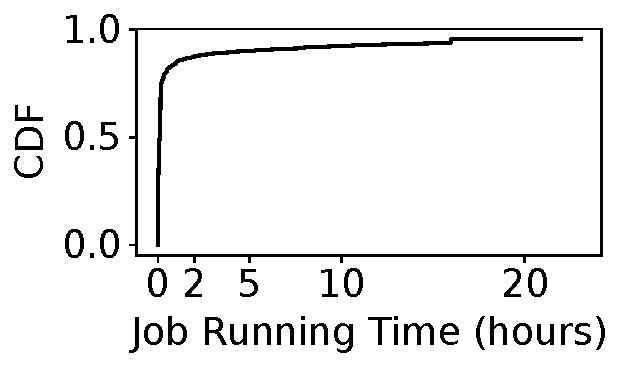
\includegraphics[width=0.2\textwidth]{../graphs/job-run-cdf.pdf}
  \vspace*{\myfigspace}
  \caption{Most HPC jobs are less than 2 hours.}
  \label{fig:job-run-cdf}
    \vspace*{\myfigspace}
\end{figure}

%%%%%%%%%%%%%%%%%%%%%%%%%%%%%%%%%%%%%%%%%%%%%%%%%%
%\vspace*{\subsecspace}
\subsubsection{Increasing Cluster Size} 

\begin{figure}
  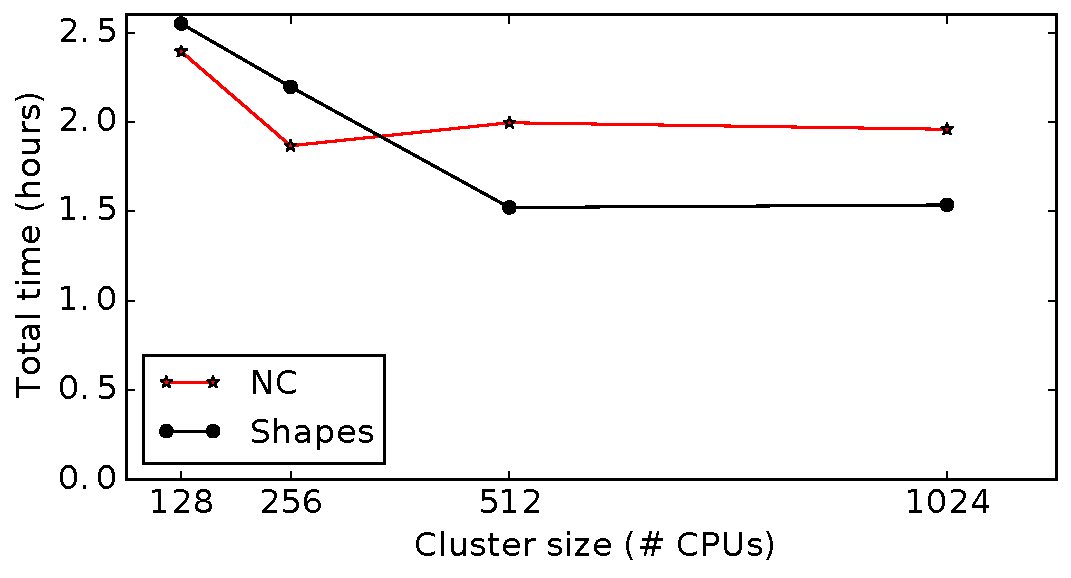
\includegraphics[width=0.4\textwidth]{../graphs/vm-per-job-scaling.pdf}
      \vspace*{\myfigspace}
  \caption{Bag of jobs running times exhibits classic parallel scaling behavior---performance improves until reaching a saturation point.}
  \label{fig:vm-per-job-scaling}
    \vspace*{\myfigspace}
\end{figure}

It is common to deploy scientific computing applications on large clusters, and we evaluate \sysname on different cluster sizes in Figure~\ref{fig:vm-per-job-scaling}.
The figure shows the total running time of the bag of jobs for the Nanoconfinement and Shapes applications as the total number of VMs (and hence total number of CPUs) increases.
For this experiment, we used \texttt{n1-highcpu-32} VMs with 32 CPUs each, and we ran four jobs in parallel on the entire cluster. 
We see classic scaling behavior: both applications can scale to a higher number of VMs up to a point, after which communication overhead starts to dominate, and the performance saturates and we see no reduction in running time. 


\begin{figure}
  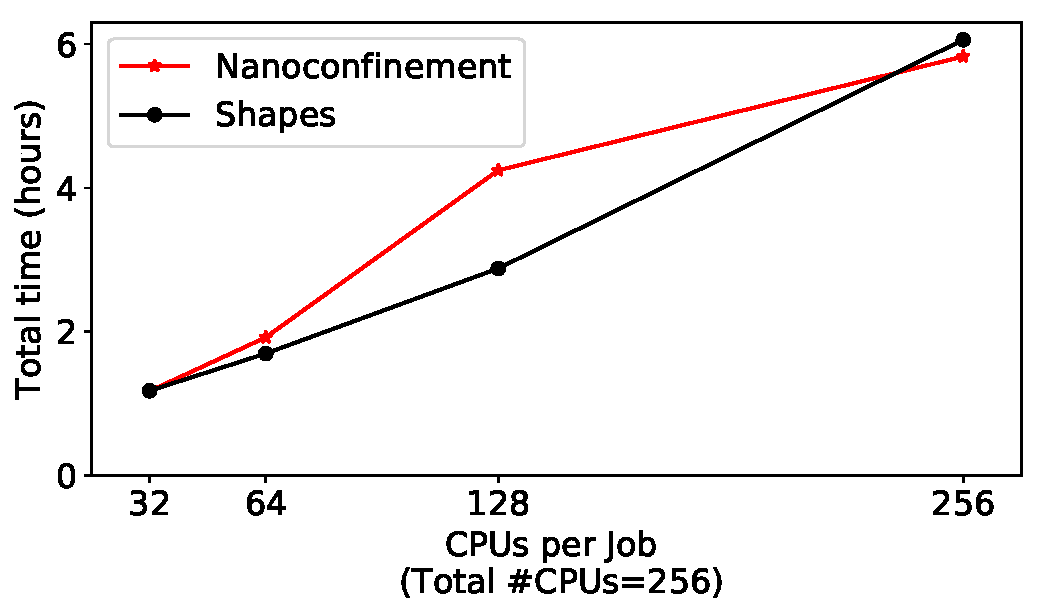
\includegraphics[width=0.2\textwidth]{../graphs/par-scaling.pdf}
      \vspace*{\myfigspace}
  \caption{\sysname can alleviate poor scaling by running more jobs in parallel and thus decreasing the intra-job parallelism (and hence number of CPUs per job, as shown in the figure).}
  \label{fig:par-scaling}
    \vspace*{\myfigspace}
\end{figure}


We note that \sysname provides the option to alleviate the parallel scaling bottleneck, by increasing the number of parallel jobs.
That is, for a given fixed cluster size, it can run more jobs in parallel, by reducing the total resources allocated and hence the parallelism 
of an individual job. 
The effect of changing the number of parallel jobs is shown in Figure~\ref{fig:par-scaling}, which shows the running time of an entire bag of jobs when the total cluster size is fixed (256 CPUs), but the number of parallel jobs and hence the number of CPUs per job changes.
We see that a \emph{smaller} number of CPUs per job limits the communication overhead, and thus reduces the total running time of the bag.
For both the NC and Shapes application, we see up to $6\times$ reduction in the total bag running time when more number of jobs are launched in parallel and a smaller number of CPUs per job are used. 


%%%%%%%%%%%%%%%%%%%%%%%%%%%%%%%%%%%%%%%%%%%%%%%%%%
\subsubsection{Increasing Bag Size}

We now evaluate \sysname's behavior when running larger bags of jobs.
Table~\ref{tab:100-jobs} shows the total running time of bags of 32 and 100 jobs.
Since \sysname reuses VMs when running jobs from a bag, it is able to take advantage of the relatively low preemption rates of VMs once they pass the first phase of early failures (Figure~\ref{fig:cdf}), and thus minimizes the number of preemptions as well as job failures. 
This makes \sysname particularly suitable for running the large bags of jobs that are required when using machine learning techniques for HPC workloads, an emerging research area in many science and engineering disciplines~\cite{ml.atomic2017,melko2017,sam2017,fu2017,long2015machine,ferguson2017machine,ward2018matminer,jcs1,jcs2,fox2019learning}, since the training and testing data needed for statistical machine learning can be generated through \sysname's bag of jobs execution model. 


%32_2_4 
\begin{table}
  \begin{tabular}{|c|r|r|r|}
    \hline
    Workload & Jobs & Time (Hours) & \# Preemptions \\
    \hline
    Nanoconfinement & 32  & 1.87 & 0 \\
    Nanoconfinement & 100  & 6.08 & 1 \\
    \hline
    Shapes & 32 & 1.47 & 0 \\
    Shapes & 100 & 4.49 & 5  \\  
    \hline
  \end{tabular}
  \caption{Running times and number of preemptions for bags of different sizes. }
  \label{tab:100-jobs}
  \vspace*{\myfigspace}
\end{table}




%%%%%%%%%%%%%%%%%%%%%%%%%%%%%%%%%%%%%%%%%%%%%%%%%%
\subsubsection{Increasing Preemptions}

By reusing VMs across a bag of jobs and taking advantage of the low preemption rates during the middle of the 24 hour life of the preemptible VMs, the \emph{expected} job failure rates and recomputation times are fairly small with \sysname (as shown in Figures~\ref{fig:runtimes-bar},~\ref{fig:hpc-vs-scispot}).
However, preemption rates can increase when the cloud operator sees high demand for resources.
Figure~\ref{fig:fails-time} shows the running time of the bag of 32 Nanoconfinement jobs on a cluster of 4 \texttt{n1-highcpu-32} VMs, when different number of VMs are preempted. 

We see that even with a high number of preemptions, the running time only increases by 50\%. 
We note that a higher than expected preemption rate (as shown in the figure) is rare, and happens with a vanishingly small likelihood. 
This shows that \sysname is robust and can provide acceptable performance even under extreme, adverse conditions. 

\begin{figure}[t]
  \centering 
  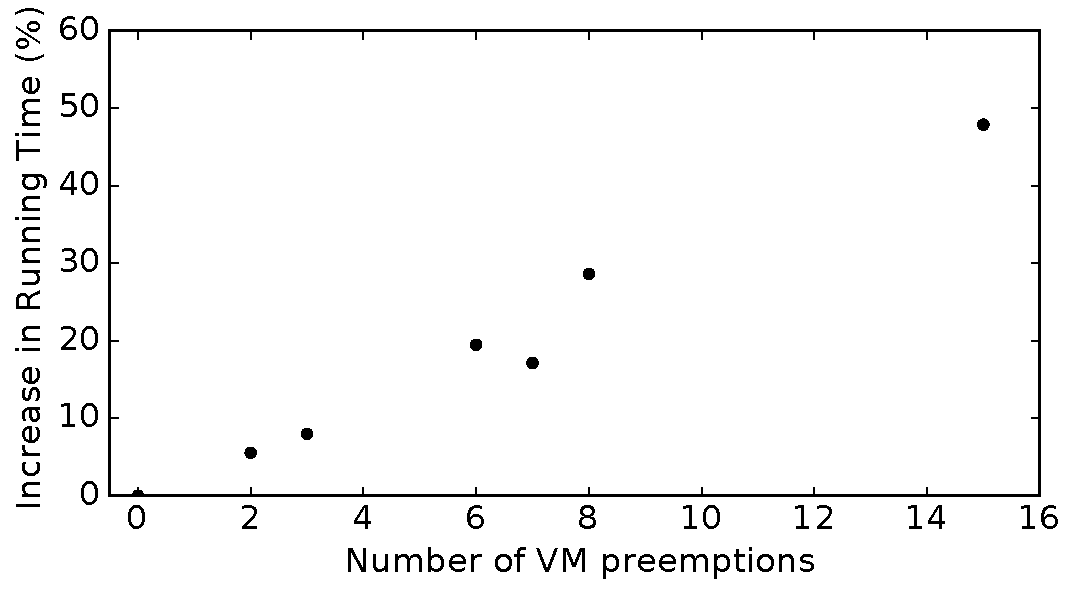
\includegraphics[width=0.2\textwidth]{../graphs/confin-fails-vs-time-relative.pdf}
      \vspace*{\myfigspace}
  \caption{The increase in running time due to preemptions is under 50\%, even when the number of preemptions is high.}
  \label{fig:fails-time}
\end{figure}


%Summary of results? 

%%%%%%%%%%%%%%%%%%%%%%%%%%%%%%%%%%%%%%%%%%%%%%%%%%


% \begin{figure}
%   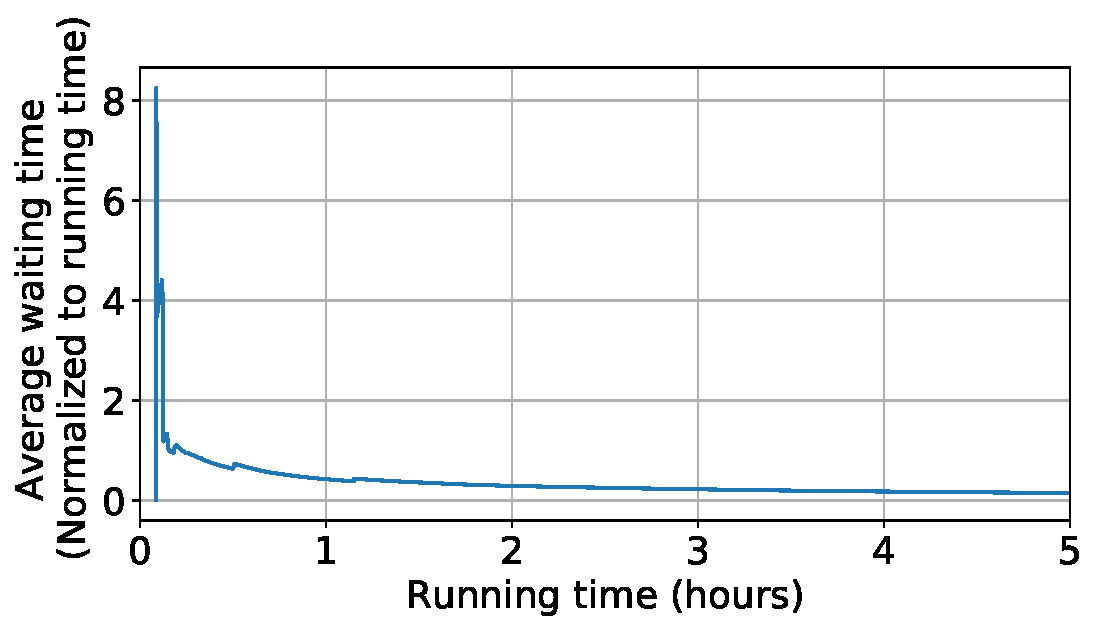
\includegraphics[width=0.4\textwidth]{../data/waiting_cumul.pdf}
%   \caption{The average waiting time (normalized to running time) of jobs of different length.}
%   \label{fig:hpc-wait-cdf}
% \end{figure}



%%% Local Variables:
%%% mode: latex
%%% TeX-master: "paper"
%%% End:
